% Chapter Template

\chapter{Implementation} % Main chapter title

\label{Chapter3} % Change X to a consecutive number; for referencing this chapter elsewhere, use \ref{ChapterX}

\lhead{Chapter 3. \emph{Chapter Title Here}} % Change X to a consecutive number; this is for the header on each page - perhaps a shortened title


\section{Mood Detection}

A common reason for engaging in music listening is that music is an effective means of conveying and evoking emotions. Although they may be subjective, based in part on the listener’s cultural and musical background or preferences, there are commonalities in perceived emotion across different listeners based on the characteristics of the music. Several studies have attempted to predict emotion conveyed during music listening. Some have explored the relationship between physiological activity experienced by a listener and perceived emotion, while others focused on the relationship between perceived emotion and the musical/acoustic features themselves. In our approach, we adapted the latter option, representing emotion using a two-dimensional space with valence on the x-axis and arousal on the y-axis.

In our exploration we decided to base our research on data collected by \cite{1000songs}, to avoid personal bias in assessing the mood of the song. The songs in the dataset were annotated by more than 300 crowdworkers on Amazon Mechanical Turk. Each song was annotated for arousal and for valence separately.

\subsection{Choice of Features}
Using Essentia library, we implemented an extractor to retrieve certain features from a song, which we would expect to have certain impact on the perceived mood of a musical piece:
\begin{itemize}
\item average loudness - dynamic range descriptor. It rescales average loudness, computed on 2sec windows with 1 sec overlap, into the [0,1] interval. The value of 0 corresponds to signals with large dynamic range, 1 corresponds to signal with little dynamic range. 
\item means and derivatives of variance of rates of silent frames in a signal for thresholds of 20, 30 and 60db,
\item dynamic complexity - dynamic complexity computed on 2sec windows with 1sec overlap
\item BMP - BPM value according to detected beats
\item spectral centroid - centroid statistics describing the spectral shape
\item spectral RMS
\item spectral energy
\item mean and derivative of variance of beat loudness -  spectral energy computed on beats segments of audio across the whole spectrum, and ratios of energy in 6 frequency bands.
\item scale and key of chords and the key
\item means of zero-crossing rate
\item pitch salience of a spectrum
\item mean and derivative of variance of dissonance. 
\end{itemize}

\begin{figure}
        \centering
        \begin{subfigure}[b]{0.48\textwidth}
                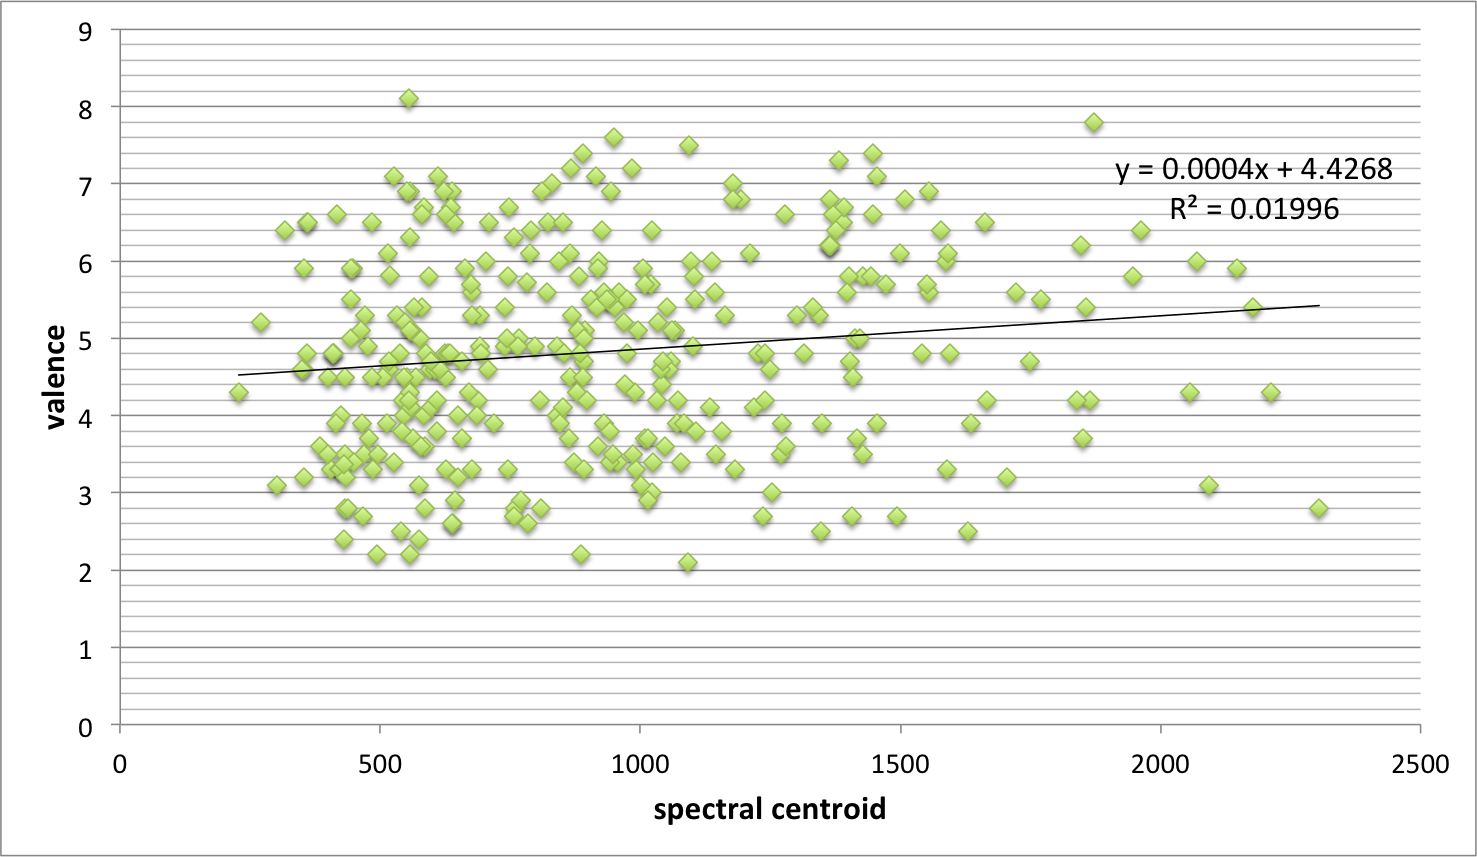
\includegraphics[width=\textwidth]{Figures/spectralcentroid-valence}
                \caption{A graph representing a correlation between spectral centroid and valence values.}
                \label{fig:is }
        \end{subfigure}%
        ~ %add desired spacing between images, e. g. ~, \quad, \qquad, \hfill etc.
          %(or a blank line to force the subfigure onto a new line)
        \begin{subfigure}[b]{0.48\textwidth}
                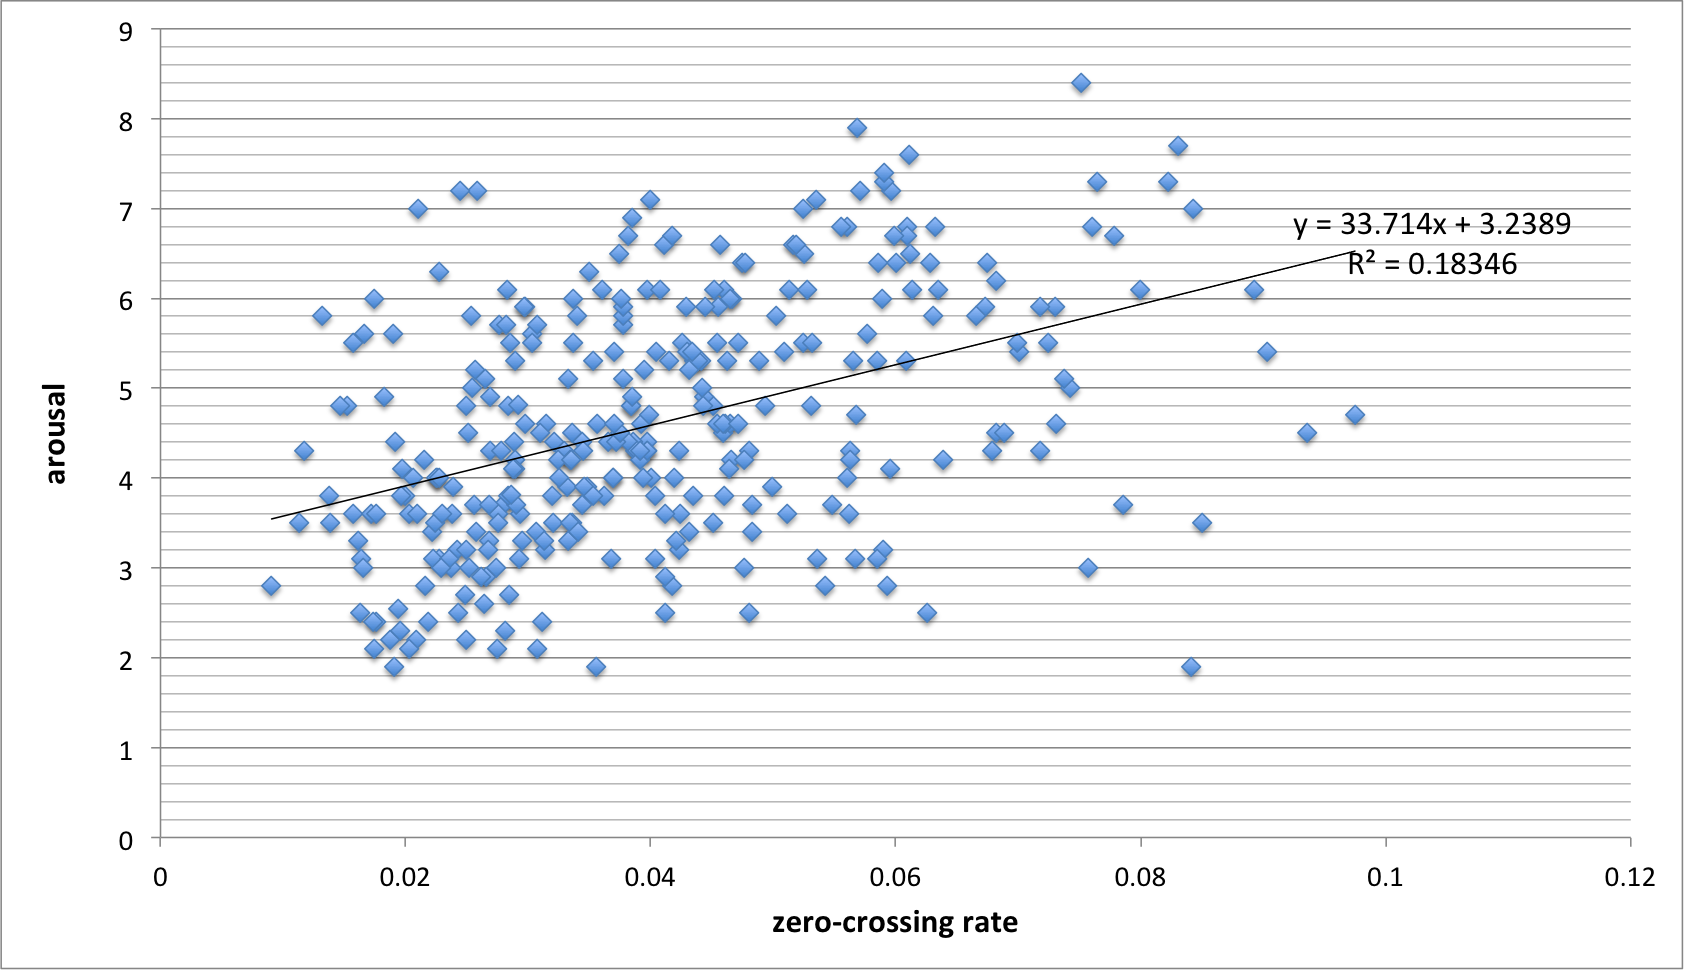
\includegraphics[width=\textwidth]{Figures/zerocrossing-arousal}
                \caption{ graph representing a correlation between zero-crossing rate and arousal values.}
                \label{fig:simtunes}
        \end{subfigure}
          \caption{Chosen results of bivariate correlation with multiple regression.}
        ~ %add desired spacing between images, e. g. ~, \quad, \qquad, \hfill etc.
\end{figure}



\subsection{Correlation between music features and music mood perception}

As a first step towards understanding the pattern by which audio features might account for emotion ratings, we conducted correlational analyses between features and mean valence/arousal ratings from the data set. We performed a bivariate correlation analysis with the valence/arousal ratings as the dependent variable, and each of the 22 features as the explanatory variable. We found significant correlation between \textit{valence} and \textit{dvar and mean silence60, dvar of silence30, dynamic complexity, spectral centroid, spectral RMS, spectral energy, zero-crossing rate, pitch salience, and both mean and dvar of dissonance}. For \textit{arousal}, we noticed correlation with \textit{spectral centroid, pitch salience, zero-crossing rate}, both \textit{mean} and \textit{dva}r of  \textit{silence60, spectral energy, mean dissonance} and \textit{dynamic complexity}.

Values of all the features were normalized between 0 and 1. 




\section{The Game}
Morbi rutrum odio eget arcu adipiscing sodales. Aenean et purus a est pulvinar pellentesque. Cras in elit neque, quis varius elit. Phasellus fringilla, nibh eu tempus venenatis, dolor elit posuere quam, quis adipiscing urna leo nec orci. Sed nec nulla auctor odio aliquet consequat. Ut nec nulla in ante ullamcorper aliquam at sed dolor. Phasellus fermentum magna in augue gravida cursus. Cras sed pretium lorem. Pellentesque eget ornare odio. Proin accumsan, massa viverra cursus pharetra, ipsum nisi lobortis velit, a malesuada dolor lorem eu neque.



\section{Main Section 2}

Sed ullamcorper quam eu nisl interdum at interdum enim egestas. Aliquam placerat justo sed lectus lobortis ut porta nisl porttitor. Vestibulum mi dolor, lacinia molestie gravida at, tempus vitae ligula. Donec eget quam sapien, in viverra eros. Donec pellentesque justo a massa fringilla non vestibulum metus vestibulum. Vestibulum in orci quis felis tempor lacinia. Vivamus ornare ultrices facilisis. Ut hendrerit volutpat vulputate. Morbi condimentum venenatis augue, id porta ipsum vulputate in. Curabitur luctus tempus justo. Vestibulum risus lectus, adipiscing nec condimentum quis, condimentum nec nisl. Aliquam dictum sagittis velit sed iaculis. Morbi tristique augue sit amet nulla pulvinar id facilisis ligula mollis. Nam elit libero, tincidunt ut aliquam at, molestie in quam. Aenean rhoncus vehicula hendrerit.